%=================================================
% CHAPITRE 1 : Cadre général du projet
%=================================================

\chapter{Cadre général du projet}

\section{Introduction}

Ce chapitre présente le projet dans son ensemble. Nous commencerons par situer le cadre dans lequel il a été réalisé, puis nous présenterons l'organisme d'accueil et le contexte métier visé. Nous exposerons ensuite la problématique, avant d'étudier l'existant et d'en dégager les limites. Enfin, nous présenterons la solution proposée, la méthodologie adoptée, l'architecture globale, l'environnement de développement ainsi que les principaux choix technologiques retenus.

\section{Présentation de l'organisme d'accueil}

\subsection{Présentation générale}

Le projet a été réalisé dans le cadre de \textbf{SmartIT}, une structure spécialisée dans la conception et le développement de solutions numériques destinées principalement aux établissements universitaires. Son activité s'inscrit dans un contexte où les universités, instituts et structures de formation cherchent à moderniser leurs outils de gestion sans perdre les règles administratives qui leur sont propres.

SmartIT accompagne ces établissements dans la mise en place d'applications capables de gérer des données sensibles, de dématérialiser certaines procédures et de faciliter le travail quotidien des services administratifs. Cette orientation a naturellement influencé le sujet de ce projet. Une solution destinée au monde universitaire ne peut pas se limiter à une gestion générique des utilisateurs ou des documents ; elle doit tenir compte de l'année universitaire, des engagements des vacataires, des structures pédagogiques, des documents officiels et des différences d'organisation entre établissements.

\subsection{Domaines d'activités}

Les domaines d'activités concernés par le projet relèvent principalement de la gestion administrative, de la gestion RH et de la production documentaire. Dans un établissement universitaire, ces domaines sont fortement liés. Les données du personnel servent à alimenter des attestations, des contrats, des justificatifs, des décisions internes ou encore des documents associés aux charges pédagogiques.

Le premier domaine concerne donc la gestion des données administratives et RH : personnel permanent, enseignants, vacataires, intervenants, modules pédagogiques, charges horaires et positions administratives. Le deuxième domaine est la production documentaire, qui exige une mise en forme fiable et conforme à l'identité de l'établissement. Le troisième domaine, plus technique mais essentiel, est la configurabilité : chaque établissement peut avoir ses propres modules, ses propres modèles de documents et ses propres règles de filtrage.

Cette diversité explique pourquoi SmartIT a besoin d'une solution souple. Un outil trop figé obligerait les développeurs à intervenir à chaque changement demandé par un établissement. À l'inverse, une plateforme configurable permettrait de mieux accompagner l'évolution des besoins sans multiplier les redéploiements.

\section{Présentation du projet}

\subsection{Cadre du projet}

SIRH-Doc s'inscrit dans le cadre de ce Projet de Fin d'Études. Il vise à concevoir et réaliser une plateforme de gestion documentaire dynamique adaptée aux établissements universitaires. Le projet prend appui sur un besoin observé dans l'existant de SmartIT : disposer d'une solution capable de produire des documents RH fiables, tout en donnant aux établissements une plus grande autonomie dans la configuration de leurs modules et de leurs modèles.

L'idée de départ n'était donc pas de créer un simple éditeur de documents. Le véritable enjeu était de construire un système qui relie les données métier, les règles d'organisation, les années universitaires et les modèles documentaires. Cette approche permet de réduire les interventions répétitives dans le code, tout en gardant un cadre technique contrôlé pour les requêtes, les filtres et l'archivage.

\subsection{Problématique}

La problématique du projet peut être formulée ainsi : \textit{comment faire évoluer une solution documentaire fortement dépendante du code vers une plateforme configurable, capable de gérer plusieurs établissements universitaires, plusieurs modules métier et plusieurs structures de documents sans redéploiement systématique ?}

Cette problématique regroupe plusieurs difficultés. Sur le plan fonctionnel, l'utilisateur doit pouvoir retrouver rapidement un bénéficiaire, choisir un modèle, générer un document fidèle et le retrouver par la suite. Sur le plan technique, le système doit remplacer une logique codée en dur par des métadonnées maîtrisées, capables de décrire les modules, les vues, les filtres, les familles documentaires et les templates. Sur le plan organisationnel, chaque établissement doit pouvoir adapter ses documents et certains paramètres sans dépendre d'une nouvelle intervention du développeur.

La difficulté réside dans l'équilibre à trouver. Une application trop rigide reproduirait les limites de l'existant. Une application trop ouverte risquerait au contraire de produire des requêtes difficiles à contrôler ou des documents incohérents. SIRH-Doc cherche à répondre à cette tension en proposant une configuration avancée, mais encadrée par une architecture claire.

\subsection{Étude de l'existant}

Avant SIRH-Doc, SmartIT disposait d'une solution appelée \textbf{DocStream}. Cette application permettait déjà de gérer certains modules et de produire des documents pour des établissements universitaires. Elle répondait donc à un besoin réel, mais son fonctionnement restait très dépendant du code source.

Dans DocStream, les modules étaient configurés manuellement par les développeurs. Lorsqu'un nouvel établissement devait être intégré, il fallait préparer une configuration spécifique, adapter les modules concernés et effectuer un nouveau déploiement. Cette manière de procéder pouvait être acceptable pour un nombre limité de cas, mais elle devenait lourde lorsque les besoins variaient d'une organisation à l'autre.

La gestion documentaire présentait la même limite. Les types de documents étaient codés en dur et la structure des documents était écrite directement dans le code. Il n'existait pas de véritable notion de template configurable par l'établissement. Les organisations pouvaient personnaliser certains éléments visibles, comme le nom de l'établissement, le logo ou quelques informations institutionnelles, mais elles ne pouvaient pas modifier librement la structure du document, réorganiser les sections, ajuster la mise en page ou créer un nouveau modèle complet sans intervention technique.

Le filtrage par année académique était également traité manuellement. Lorsqu'une table devait être filtrée par année universitaire, la règle devait être prévue explicitement dans le code. De la même façon, les modules disponibles étaient prédéfinis. Si un établissement souhaitait ajouter un nouveau module ou modifier profondément une logique existante, il fallait modifier l'application puis la redéployer.

Ce constat a mis en évidence une limite importante : DocStream fonctionnait, mais son évolution reposait trop fortement sur les développeurs. Pour un produit destiné à plusieurs établissements universitaires, cette dépendance rendait la maintenance plus coûteuse et ralentissait la personnalisation.

\subsection{Solution proposée}

Face à ces limites, SIRH-Doc propose une plateforme web plus configurable. Elle reprend l'objectif général de DocStream, à savoir produire des documents à partir de données métier, mais elle le fait avec une architecture pensée pour réduire les modifications directes du code. La solution repose sur un backend ASP.NET Core, un frontend Angular et des bases SQL Server séparant l'authentification, la configuration et les données tenant.

Le premier apport concerne le contexte et la sécurité. L'utilisateur s'authentifie par JWT, puis le middleware de résolution tenant identifie son organisation et initialise le contexte utilisé par les services et repositories. L'année universitaire active est également prise en compte afin que les tables historiques soient filtrées lorsque la configuration l'exige.

Le deuxième apport est le moteur dynamique de données. Les modules, les vues de tables, les colonnes visibles, les filtres et les listes de valeurs sont décrits par des métadonnées. Ainsi, l'ajout d'un module ou l'adaptation d'une vue ne nécessite plus systématiquement une modification du code. Cette approche demande une configuration rigoureuse, mais elle répond directement au besoin d'adaptabilité.

Le troisième apport concerne le studio documentaire. Les familles documentaires définissent les sources de données, les templates décrivent la structure des documents et les chartes graphiques portent l'identité visuelle de l'organisation. Les documents ne sont donc plus entièrement figés dans le code. L'établissement gagne une marge de personnalisation plus large, tout en conservant un moteur de fusion contrôlé.

Enfin, SIRH-Doc intègre un module d'archivage. Chaque document généré conserve son contenu final et ses métadonnées : famille, template, bénéficiaire, générateur, organisation et date. Cette traçabilité est indispensable dans un contexte RH, car un document administratif doit pouvoir être retrouvé et justifié après sa production.

\section{Méthodologies adoptées}

Dans l’optique de garantir une évolution progressive et maîtrisée du projet, nous avons adopté la méthode Agile Scrum.

\begin{itemize}

    \item \textbf{Scrum Agile}

    La méthodologie Scrum Agile est une approche de gestion de projet basée sur des cycles itératifs appelés sprints, généralement d’une durée de 2 à 4 semaines, visant à livrer un produit fonctionnel à chaque fin de cycle.

    L’équipe Scrum se compose du Product Owner, qui définit les priorités et gère le backlog produit ; du Scrum Master, qui veille au respect des principes Scrum et accompagne l’équipe ; et de l’équipe de développement, chargée de réaliser les tâches assignées.

    Chaque sprint débute par une phase de planification, suivie de réunions quotidiennes permettant de suivre l’avancement du travail. Il se termine par une revue de sprint, durant laquelle les résultats sont présentés, ainsi qu’une rétrospective visant à analyser le processus et à identifier des pistes d’amélioration.

    Scrum repose sur trois principes fondamentaux : la transparence, l’inspection et l’adaptation. Ces principes favorisent une amélioration continue et une grande réactivité face aux changements, ce qui en fait une méthode particulièrement adaptée aux projets complexes et évolutifs.

    \item \textbf{Artefacts Scrum}

    À savoir, les artefacts Scrum sont des éléments essentiels permettant d’organiser et de suivre l’avancement du projet. Ils comprennent :

    \begin{itemize}
        \item \textbf{Backlog produit :} liste priorisée des fonctionnalités et exigences à réaliser, gérée par le Product Owner.
        
        \item \textbf{Backlog de sprint :} sous-ensemble des tâches sélectionnées à partir du backlog produit et à réaliser durant un sprint donné.
        
        \item \textbf{Incrément :} ensemble des fonctionnalités terminées et potentiellement livrables à la fin de chaque sprint, représentant le produit dans son état fonctionnel.
    \end{itemize}

    \item \textbf{Implémentation de la méthodologie Scrum}

Dans le cadre de ce projet, le rôle de Product Owner a été assuré par Monsieur Anis Kricha, tandis que Monsieur Karim Kalti a occupé le rôle de Scrum Master. De mon côté, j’ai intégré l’équipe de développement en tant que membre chargé de la réalisation des fonctionnalités techniques, accompagné de Monsieur Gharbi Ahmed.

Cette organisation a permis de structurer efficacement le suivi du projet et de garantir l’application des principes de la méthode Scrum tout au long du développement. Le Product Owner était responsable de la définition et de la priorisation des besoins, tandis que le Scrum Master veillait au respect du cadre méthodologique et à la fluidité du processus de travail.

Sous cette coordination, nous avons travaillé à la concrétisation des fonctionnalités définies dans le backlog produit, en les transformant progressivement en incréments fonctionnels à chaque sprint. Cette approche itérative a permis d’assurer une meilleure visibilité sur l’avancement du projet et d’ajuster régulièrement les priorités en fonction des contraintes techniques et des besoins exprimés.

La communication régulière entre les membres de l’équipe a joué un rôle essentiel dans la réussite du projet. Elle a permis d’identifier rapidement les obstacles, de les résoudre de manière collaborative et d’adapter le plan de travail afin de respecter les délais tout en garantissant la qualité des livrables.

    \begin{figure}[H]
        \centering
        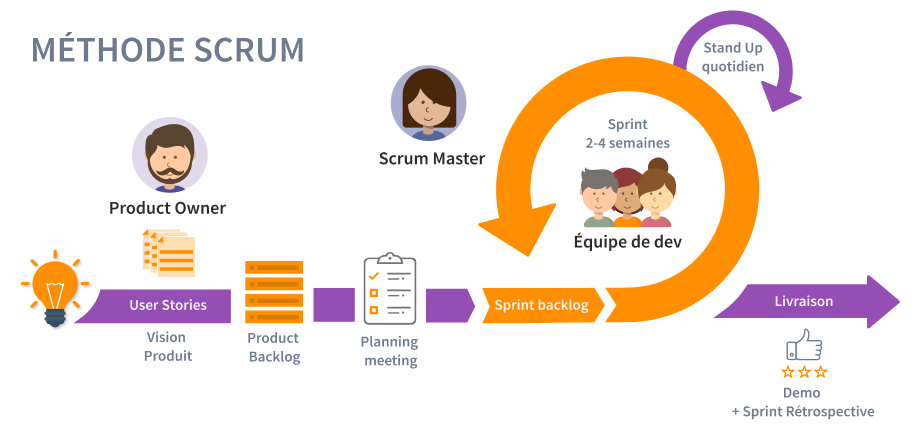
\includegraphics[width=0.9\textwidth]{images/scrum-process-schema.png}
        \caption{Méthodologie SCRUM}
        \label{fig:scrum-methodology}
    \end{figure}

\end{itemize}

\subsection{Langage de Modélisation Unifié UML}

Le langage de modélisation unifié UML (Unified Modeling Language) est un
langage de modélisation standardisé, largement adopté en ingénierie logicielle pour
concevoir, visualiser, spécifier et documenter les systèmes complexes.

\section{Architecture globale de l'application}

L'architecture d'une application donne une vision claire de la manière dont ses différentes parties collaborent. Dans SIRH-Doc, elle devait surtout répondre à trois besoins : isoler les établissements, maintenir une logique métier maîtrisée et permettre l'évolution des modules sans remettre en cause l'ensemble du système. Pour cela, nous avons retenu une architecture physique en \textbf{3-tiers}, complétée par une organisation logique inspirée de la \textbf{Clean Architecture}.

\subsection{Architecture physique}

Physiquement, SIRH-Doc suit une organisation classique à trois niveaux. Le premier niveau est le \textbf{client web}, développé avec Angular, qui porte l'interface utilisateur. Le deuxième est le \textbf{serveur d'application}, développé avec ASP.NET Core, où sont traitées les règles sensibles comme l'authentification, la résolution du tenant ou la génération documentaire. Le troisième est le \textbf{serveur de base de données}, basé sur SQL Server.

Cette séparation reste simple mais structurante pour le projet. Le navigateur ne communique jamais directement avec la base de données ; il passe systématiquement par l'API, qui contrôle le contexte utilisateur et applique les règles de sécurité. Les données sont ainsi organisées selon leur rôle : authentification, configuration système et données propres à chaque établissement.

\begin{figure}[H]
    \centering
    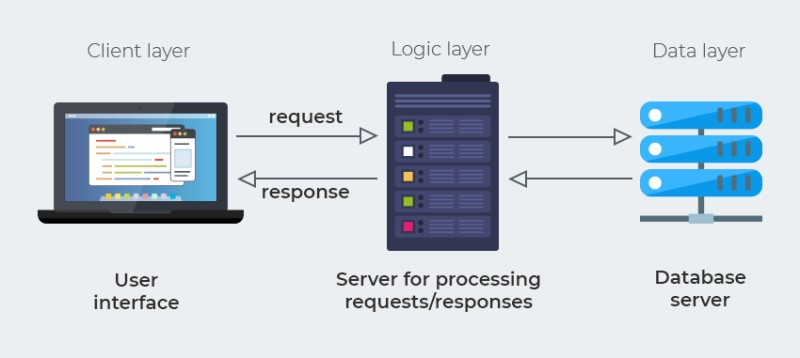
\includegraphics[width=0.95\textwidth]{images/architecture-physique.png}
    \caption{Architecture physique de l'application}
    \label{fig:architecture-physique}
\end{figure}

\subsection{Architecture logique}

Sur le plan logique, le backend s'inspire des principes de la \textbf{Clean Architecture}. Cette approche structure l'application en couches distinctes : les contrôleurs exposent les endpoints de l'API, les services encapsulent la logique métier, les entités représentent le cœur du domaine, et les repositories gèrent l'accès aux données.

Cette séparation permet d’éviter le mélange entre règles métier et détails techniques, ce qui améliore la maintenabilité et l’évolutivité du système.

Dans SIRH-Doc, ce choix s’est révélé particulièrement pertinent, car plusieurs traitements traversent l’ensemble de l’application : le multi-tenant, le filtrage par année universitaire, les modules dynamiques et l’archivage documentaire. Par exemple, le middleware de résolution du tenant initialise le contexte de l’utilisateur avant l’exécution des services, garantissant ainsi une exécution cohérente des règles métier.

\begin{figure}[H]
    \centering
    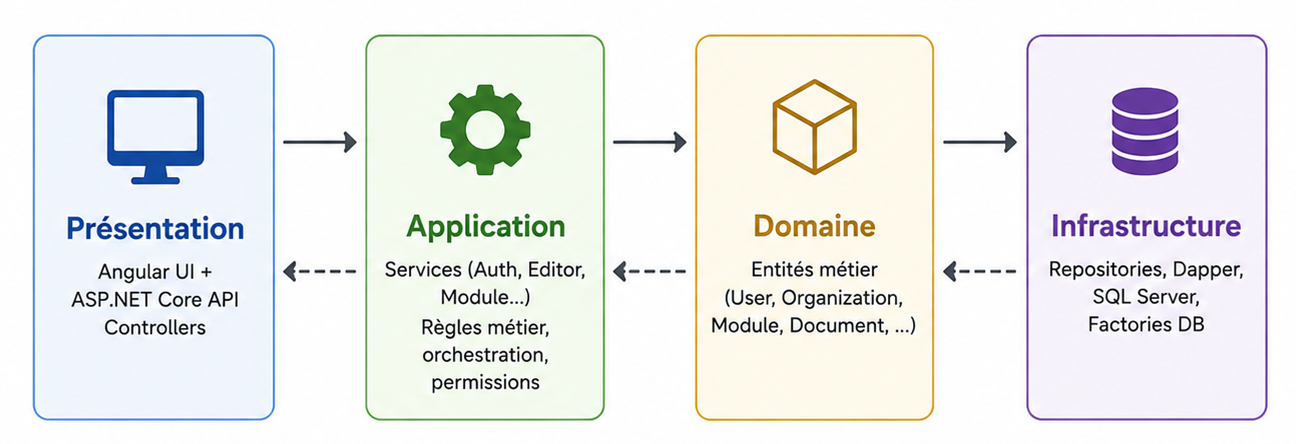
\includegraphics[width=0.95\textwidth]{images/architecture-logique.png}
    \caption{Architecture logique basée sur Clean Architecture}
    \label{fig:architecture-logique}
\end{figure}


\section{Environnement de développement}

\subsection{Environnement matériel}

\begin{table}[H]
\centering
\renewcommand{\arraystretch}{1.3}
\begin{tabular}{|l|l|}
\hline
\textbf{Type} & PC Portable Lenovo LOQ \\
\hline
\textbf{Processeur} & Intel Core i7-13650HX \\
\hline
\textbf{Mémoire RAM} & 32 Go DDR5 \\
\hline
\textbf{Système d’exploitation} & Windows 11 \\
\hline
\textbf{Stockage} & SSD 512 Go \\
\hline
\end{tabular}
\caption{Tableau descriptif de l’infrastructure matérielle utilisée}
\label{tab:env-materiel}
\end{table}

\subsection{Environnement logiciel}

Le développement de SIRH-Doc s'est appuyé sur un ensemble d'outils simples mais complémentaires. Ils ont servi à écrire le code, tester l'application, administrer les bases de données et produire les diagrammes du rapport.

% Taille uniforme des logos
\newcommand{\logoSize}{1.8cm}

\begin{table}[H]
\centering
\renewcommand{\arraystretch}{1.5}

\begin{tabular}{|>{\centering\arraybackslash}m{3cm}|m{11cm}|}
\hline
\textbf{Outil} & \textbf{Description} \\
\hline

\centering
\IfFileExists{images/logos/chrome.png}
{
\includegraphics[width=\logoSize,height=\logoSize,keepaspectratio]{images/logos/chrome.png}}
{\fbox{\parbox[c][\logoSize][c]{2cm}{\centering Chrome}}}
&
\textbf{Google Chrome :} Chrome a été utilisé comme navigateur principal pour tester l'application Angular, vérifier le rendu des interfaces, contrôler les formulaires dynamiques et valider les parcours de génération documentaire.
\\
\hline

\centering
\IfFileExists{images/logos/vscode.png}
{
\includegraphics[width=\logoSize,height=\logoSize,keepaspectratio]{images/logos/vscode.png}}
{\fbox{\parbox[c][\logoSize][c]{2cm}{\centering VS Code}}}
&
\textbf{Visual Studio Code :} Visual Studio Code a servi d'environnement de développement principal pour le backend ASP.NET Core, le frontend Angular et les fichiers du rapport. Ses extensions ont facilité la navigation dans le projet, l'édition TypeScript/C\# et la gestion des fichiers LaTeX.
\\
\hline

\centering
\IfFileExists{images/logos/dbeaver.png}
{
\includegraphics[width=\logoSize,height=\logoSize,keepaspectratio]{images/logos/dbeaver.png}}
{\fbox{\parbox[c][\logoSize][c]{2cm}{\centering DBeaver}}}
&
\textbf{DBeaver CE :} DBeaver Community Edition a été utilisé pour consulter et administrer les bases SQL Server. Il a permis de vérifier les tables, tester certaines requêtes SQL et contrôler les données liées aux organisations, aux configurations et aux archives.
\\
\hline

\centering
\IfFileExists{images/logos/drawio.png}
{
\includegraphics[width=\logoSize,height=\logoSize,keepaspectratio]{images/logos/drawio.png}}
{\fbox{\parbox[c][\logoSize][c]{2cm}{\centering Draw.io}}}
&
\textbf{Draw.io :} Draw.io a été utilisé pour réaliser les diagrammes UML du projet : diagrammes de classes, cas d'utilisation et séquences. Son format \texttt{.drawio} a facilité les corrections progressives pendant la rédaction du rapport.
\\
\hline

\centering
\IfFileExists{images/logos/github.png}
{
\includegraphics[width=\logoSize,height=\logoSize,keepaspectratio]{images/logos/github.png}}
{\fbox{\parbox[c][\logoSize][c]{2cm}{\centering GitHub}}}
&
\textbf{GitHub :} GitHub a été utilisé pour l'hébergement du code source et le suivi des versions du projet. Il a permis de conserver l'historique des modifications et de sécuriser l'évolution progressive du backend, du frontend et des fichiers du rapport.
\\
\hline

\centering
\IfFileExists{images/logos/swagger.png}
{
\includegraphics[width=\logoSize,height=\logoSize,keepaspectratio]{images/logos/swagger.png}}
{\fbox{\parbox[c][\logoSize][c]{2cm}{\centering Swagger}}}
&
\textbf{Swagger :} Swagger a été utilisé pour visualiser et tester les endpoints exposés par le backend ASP.NET Core, notamment les routes d'authentification, de configuration, de requêtes dynamiques et d'archives.
\\
\hline

\end{tabular}

\caption{Environnement logiciel utilisé}
\label{tab:env-logiciel}

\end{table}


\section{Choix technologiques}

Les technologies retenues pour SIRH-Doc ont été choisies en fonction de la nature du projet : une application web administrative, multi-tenant, fortement liée aux données SQL Server et à la génération documentaire. Le choix ne s'est donc pas limité à la popularité des outils ; il fallait surtout disposer d'un socle stable, maintenable et suffisamment souple pour supporter les modules dynamiques.

% Taille uniforme des logos
\newcommand{\logoSize}{1.8cm}

\begin{table}[H]
\centering
\renewcommand{\arraystretch}{1.5}

\begin{tabular}{|>{\centering\arraybackslash}m{3cm}|m{11cm}|}
\hline
\textbf{Technologie} & \textbf{Rôle dans le projet} \\
\hline

\centering
\IfFileExists{images/logos/dotnet.png}
{
\includegraphics[width=\logoSize,height=\logoSize,keepaspectratio]{images/logos/dotnet.png}}
{\fbox{\parbox[c][\logoSize][c]{2cm}{\centering .NET}}}
&
\textbf{ASP.NET Core 8 :} ASP.NET Core a été utilisé pour développer l'API backend. Il offre une structure claire pour organiser les contrôleurs, les services, l'injection de dépendances, l'authentification JWT et les middlewares, notamment celui chargé de la résolution du tenant.
\\
\hline

\centering
\IfFileExists{images/logos/csharp.png}
{
\includegraphics[width=\logoSize,height=\logoSize,keepaspectratio]{images/logos/csharp.png}}
{\fbox{\parbox[c][\logoSize][c]{2cm}{\centering C\#}}}
&
\textbf{C\# :} C\# a été utilisé côté backend pour implémenter les règles applicatives, les DTOs, les entités et les services. Son typage fort aide à garder un code plus sûr dans une application qui manipule plusieurs contextes de données et de nombreuses configurations.
\\
\hline

\centering
\IfFileExists{images/logos/angular.png}
{
\includegraphics[width=\logoSize,height=\logoSize,keepaspectratio]{images/logos/angular.png}}
{\fbox{\parbox[c][\logoSize][c]{2cm}{\centering Angular}}}
&
\textbf{Angular 17 :} Angular a été choisi pour construire l'interface web. Il convient bien à une application de gestion composée de plusieurs pages, formulaires, services partagés et composants réutilisables, comme le studio documentaire, les modules dynamiques et les archives.
\\
\hline

\centering
\IfFileExists{images/logos/typescript.png}
{
\includegraphics[width=\logoSize,height=\logoSize,keepaspectratio]{images/logos/typescript.png}}
{\fbox{\parbox[c][\logoSize][c]{2cm}{\centering TypeScript}}}
&
\textbf{TypeScript :} TypeScript a permis de mieux structurer le code frontend. Il facilite la manipulation des objets de configuration, des réponses API, des modèles de templates et des données nécessaires à la prévisualisation des documents.
\\
\hline

\centering
\IfFileExists{images/logos/microsoftsqlserver.png}
{
\includegraphics[width=\logoSize,height=\logoSize,keepaspectratio]{images/logos/microsoftsqlserver.png}}
{\fbox{\parbox[c][\logoSize][c]{2cm}{\centering SQL Server}}}
&
\textbf{SQL Server :} SQL Server a été retenu pour stocker les données d'authentification, les métadonnées de configuration et les données propres aux établissements. Il répond bien aux besoins du projet, notamment les jointures, la pagination, les filtres dynamiques et les requêtes utilisées dans la génération documentaire.
\\
\hline

\centering
\IfFileExists{images/logos/html5.png}{
    
\includegraphics[width=0.85cm,height=0.85cm,keepaspectratio]{images/logos/html5.png}
    \hspace{0.15cm}
    
\includegraphics[width=0.85cm,height=0.85cm,keepaspectratio]{images/logos/scss.png}
}{
    \fbox{\parbox[c][\logoSize][c]{2cm}{\centering HTML/SCSS}}
}
&
\textbf{HTML et SCSS :} HTML et SCSS ont été utilisés pour structurer et mettre en forme les interfaces. Ils ont permis d'adapter les pages aux usages administratifs du projet : tableaux, formulaires, filtres, éditeur, sélection de l'année universitaire et consultation des archives.
\\
\hline

\end{tabular}

\caption{Langages et technologies de développement utilisés}
\label{tab:technologies-dev}

\end{table}

\section{Conclusion}

Ce chapitre a présenté le cadre général du projet, depuis le contexte de SmartIT jusqu'aux choix méthodologiques et technologiques. L'étude de l'existant a montré les limites de DocStream, notamment la dépendance au code, les redéploiements fréquents et la faible personnalisation documentaire. La solution proposée, SIRH-Doc, vise à dépasser ces limites grâce à une architecture configurable, multi-tenant et orientée métadonnées. Le chapitre suivant sera consacré à l'analyse des besoins, aux acteurs du système, au backlog produit et à la modélisation globale de la plateforme.
